\documentclass[tikz,border=1.35mm]{standalone}

\definecolor{fvmadaptedge}{HTML}{8A7E7E}
\usetikzlibrary{arrows.meta}

\definecolor{splitred}{HTML}{AF2525}

% Quadrilateral face before and after isotropic face splitting.
% Coordinates are in millimeters; y=-1mm keeps the SVG-style origin at top left.
\begin{document}
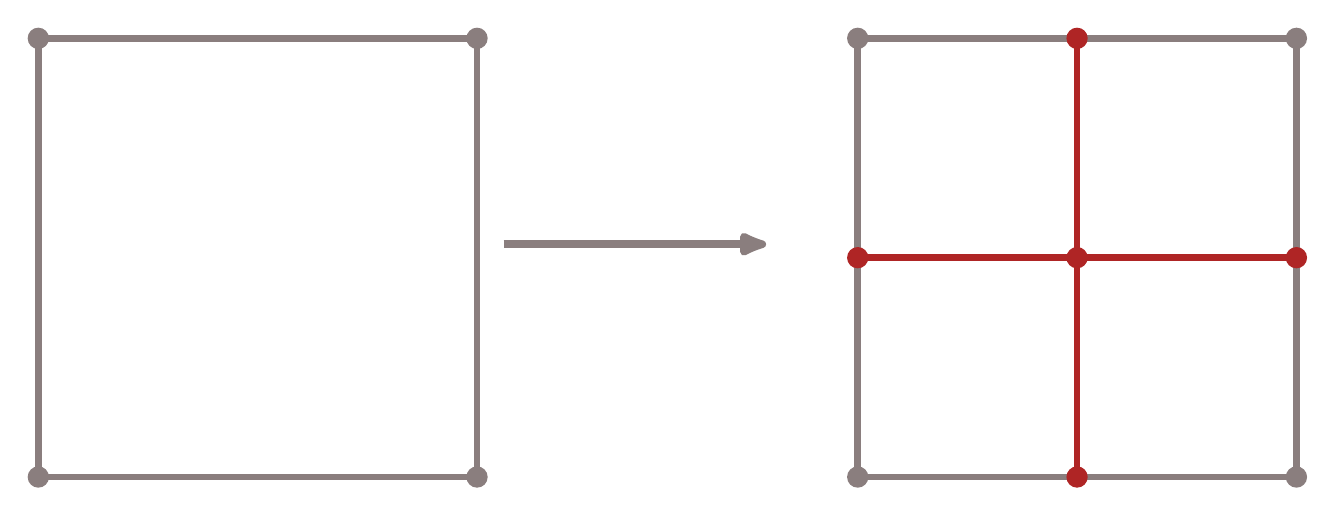
\begin{tikzpicture}[
  x=1mm,
  y=-1mm,
  line join=round,
  edge/.style={draw=fvmadaptedge,line width=0.865mm},
  splitline/.style={draw=splitred,line width=0.865mm},
  arrow/.style={draw=fvmadaptedge,line width=1.05mm,-{Latex[round,length=4.8mm,width=3.6mm]}}
]
  % Match the original artwork frame before the standalone border is applied.
  \useasboundingbox (0,0) rectangle (162.482,58.419);

  % Left panel: original unsplit quadrilateral.
  \coordinate (left0) at (1.353,1.353);
  \coordinate (left1) at (57.067,1.353);
  \coordinate (left2) at (57.067,57.067);
  \coordinate (left3) at (1.353,57.067);

  % Right panel: edge midpoints and face center created by the split.
  \coordinate (right0) at (105.415,1.353);
  \coordinate (right1) at (161.129,1.353);
  \coordinate (right2) at (161.129,57.067);
  \coordinate (right3) at (105.415,57.067);
  \coordinate (topMid) at (133.272,1.353);
  \coordinate (rightMid) at (161.129,29.210);
  \coordinate (bottomMid) at (133.272,57.067);
  \coordinate (leftMid) at (105.415,29.210);
  \coordinate (center) at (133.272,29.210);

  % Draw the old face and the split face topology.
  \draw[edge] (left0) rectangle (left2);
  \draw[edge] (right0) rectangle (right2);
  \draw[splitline] (center) -- (leftMid);
  \draw[splitline] (center) -- (rightMid);
  \draw[splitline] (center) -- (topMid);
  \draw[splitline] (center) -- (bottomMid);

  % Transformation arrow between the before/after panels.
  \draw[arrow] (60.450,27.503) -- (93.780,27.503);

  % Original vertices are #8a7e7e.
  \fill[fvmadaptedge] (left0) circle[radius=1.353mm];
  \fill[fvmadaptedge] (left1) circle[radius=1.353mm];
  \fill[fvmadaptedge] (left2) circle[radius=1.353mm];
  \fill[fvmadaptedge] (left3) circle[radius=1.353mm];

  \fill[fvmadaptedge] (right0) circle[radius=1.353mm];
  \fill[fvmadaptedge] (right1) circle[radius=1.353mm];
  \fill[fvmadaptedge] (right2) circle[radius=1.353mm];
  \fill[fvmadaptedge] (right3) circle[radius=1.353mm];

  % Split-created edge and face nodes are red.
  \fill[splitred] (topMid) circle[radius=1.353mm];
  \fill[splitred] (rightMid) circle[radius=1.353mm];
  \fill[splitred] (bottomMid) circle[radius=1.353mm];
  \fill[splitred] (leftMid) circle[radius=1.353mm];
  \fill[splitred] (center) circle[radius=1.353mm];
\end{tikzpicture}
\end{document}
